% Generated from the public primitive catalog. Original Atlas drawing; Apache-2.0.
% Target: chacha20; view: overview
\documentclass[border=9pt]{standalone}
% Original Atlas figure theme. Apache-2.0; see the repository LICENSE.
\usepackage[T1]{fontenc}
\usepackage{lmodern}
\usepackage{amsmath,amssymb}
\usepackage{tikz}
\usetikzlibrary{arrows.meta,positioning,calc,fit,backgrounds,decorations.pathreplacing,matrix}
\definecolor{atlasInk}{HTML}{172235}
\definecolor{atlasTeal}{HTML}{0D7B7D}
\definecolor{atlasMuted}{HTML}{637278}
\definecolor{atlasFill}{HTML}{EAF4F2}
\definecolor{atlasLine}{HTML}{B6C8C7}
\tikzset{
  every picture/.style={line width=.65pt,draw=atlasInk,>=Latex},
  every node/.style={text=atlasInk,font=\sffamily\small},
  box/.style={draw,rounded corners=1.5pt,minimum height=.9cm,minimum width=1.6cm,align=center,inner sep=6pt,fill=white},
  accent/.style={box,draw=atlasTeal,fill=atlasFill},
  wire/.style={->,line width=.7pt},
  keywire/.style={wire,draw=atlasTeal,dashed},
  xor/.style={draw,circle,fill=white,inner sep=0pt,minimum size=.38cm},
  add/.style={draw,rectangle,fill=white,inner sep=0pt,minimum size=.38cm},
  note/.style={font=\sffamily\scriptsize,text=atlasMuted,align=center},
  phase/.style={font=\sffamily\small\bfseries,text=atlasTeal},
  group/.style={draw=atlasLine,dashed,rounded corners=2pt,inner sep=8pt}
}
\newcommand{\rotl}{\mathbin{\lll}}
\newcommand{\rotr}{\mathbin{\ggg}}
\newcommand{\kx}{\operatorname{Keccak}\!\text{-}\!f[1600]}

\newcommand{\AtlasKeyBits}{256}
\newcommand{\AtlasKeyWords}{8}
\newcommand{\AtlasRounds}{20}
\newcommand{\AtlasPriorRounds}{19}
\newcommand{\AtlasRoundKeys}{21}
\newcommand{\AtlasDoubleRounds}{10}
\newcommand{\AtlasSixRoundGroups}{3.3333333333333335}
\newcommand{\AtlasFLGroups}{2.3333333333333335}
\newcommand{\AtlasRoundStart}{4}
\newcommand{\AtlasBlockBits}{b}
\newcommand{\AtlasOutputBits}{d}
\newcommand{\AtlasStateBits}{512}
\newcommand{\AtlasNonceBits}{96}
\newcommand{\AtlasCounterBits}{32}
\newcommand{\AtlasStreamBlockBits}{512}
\newcommand{\AtlasRate}{r}
\newcommand{\AtlasCapacity}{c}
\newcommand{\AtlasSteps}{N}
\newcommand{\AtlasLastStep}{N-1}
\newcommand{\AtlasWordBits}{64}
\newcommand{\AtlasHashWords}{16}
\newcommand{\AtlasFeedForward}{\boxplus}
\newcommand{\AtlasByteOrder}{big-endian}
\newcommand{\AtlasDomain}{01}
\newif\ifAtlasXof
\AtlasXoffalse
\begin{document}
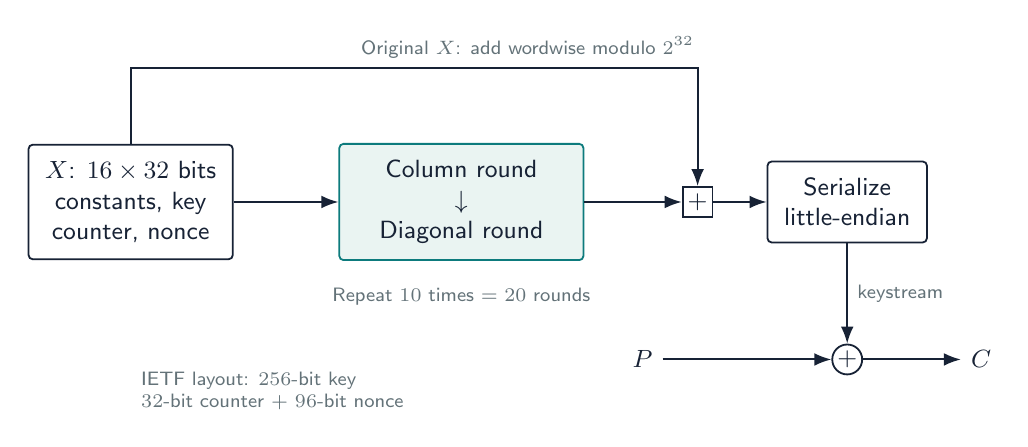
\begin{tikzpicture}
  \node[box,minimum width=2.4cm] (state) at (1.2,0) {$X$: $16\times32$ bits\\constants, key\\counter, nonce};
  \node[accent,minimum width=3.1cm] (rounds) at (5.4,0) {Column round\\$\downarrow$\\Diagonal round};
  \node[add] (sum) at (8.4,0) {$+$};
  \node[box] (ser) at (10.3,0) {Serialize\\little-endian};
  \draw[wire] (state) -- (rounds); \draw[wire] (rounds) -- (sum); \draw[wire] (sum) -- (ser);
  \draw[wire] (state.north) -- (1.2,1.7) -| node[pos=.35,above,note] {Original $X$: add wordwise modulo $2^{32}$} (sum.north);
  \node[note] at (5.4,-1.2) {Repeat $10$ times $=20$ rounds};
  \node[xor] (enc) at (10.3,-2) {$+$};
  \node (p) at (7.7,-2) {$P$}; \node (c) at (12,-2) {$C$};
  \draw[wire] (ser) -- node[right,note] {keystream} (enc);
  \draw[wire] (p) -- (enc); \draw[wire] (enc) -- (c);
  \node[note,align=left] at (3,-2.4) {IETF layout: $256$-bit key\\$32$-bit counter $+$ $96$-bit nonce};
\end{tikzpicture}

\end{document}
